\subsection{Bayer filter}
To capture color images conventional cameras use \glspl{cfa}.
The most common type of \gls{cfa} is the Bayer pattern where green pixels cover half the array in a lattice, and the red and blue pixel locations are spaced between the green pixels as shown in Figure \ref{fig:bayer_pattern} \cite{getreuerMalvarHeCutlerLinearImage2011}.
Different orderings of the colors in the \gls{cfa} exists, with the most common ones being RGGB, BGGR, GRBG, and GBRG where the letters designate the order of the four top left pixeld in the image.

\begin{figure}[tb]
    \centering
    \begin{tabular}[b]{ccc}
        \subcaptionbox{RGGB bayer pattern}{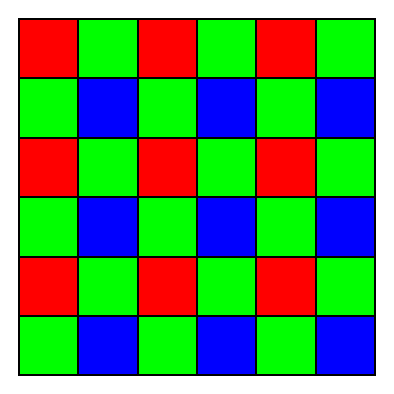
\includegraphics[width=0.25\textwidth]{figures/debayer/bayer_pattern_small.pdf}
            \label{fig:bayer_pattern}
        }                                                                                                              &
        \subcaptionbox{Green at red}{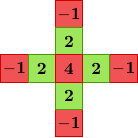
\includegraphics[width=0.25\linewidth]{figures/debayer/g_at_r.png}}               &
        \subcaptionbox{Green at red}{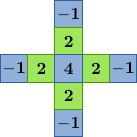
\includegraphics[width=0.25\textwidth]{figures/debayer/g_at_b.png}}                 \\
        \subcaptionbox{Red at }{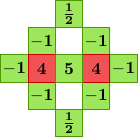
\includegraphics[width=0.25\textwidth]{figures/debayer/r_at_g_rr.png}}                 &
        \subcaptionbox{Red at green, blue row}{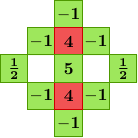
\includegraphics[width=0.25\textwidth]{figures/debayer/r_at_g_br.png}}  &
        \subcaptionbox{Red at blue}{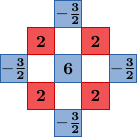
\includegraphics[width=0.25\textwidth]{figures/debayer/r_at_b.png}}                  \\
        \subcaptionbox{Blue at green, red row}{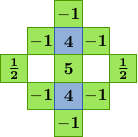
\includegraphics[width=0.25\textwidth]{figures/debayer/b_at_g_rr.png}}  &
        \subcaptionbox{Blue at green, blue row}{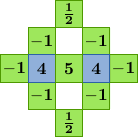
\includegraphics[width=0.25\textwidth]{figures/debayer/b_at_g_br.png}} &
        \subcaptionbox{Blue at red}{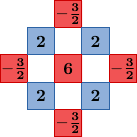
\includegraphics[width=0.25\textwidth]{figures/debayer/b_at_r.png}}
    \end{tabular}
    \caption{Bayer pattern and coefficient values used by Malvar-He-Cutler scaled by 8 \cite{getreuerMalvarHeCutlerLinearImage2011}\cite{CommonsBayerPattern2020}}
    \label{fig:debayer:malvar_filters}
\end{figure}

\subsection{Image demosaicing}
Image demosaicing is the process of estimating full-resolution color information for an image that has been captured with a bayer pattern \cite{liImageDemosaicingSystematic2008}, e.g. at each red pixel in the \gls{cfa} the green and blue intensities needs to be estimated.
Simple methods, such nearest neighbours or linear interpolation, are prone to yielding images false colors and the checkboard like patterns called the zipper effect as shown in Figure \ref{fig:artifacts_gioia} \cite{gioiaDataDrivenConvolutionalModel2021} \cite{liImageDemosaicingSystematic2008}.
A multitude of more advanced methods have been proposed with increasing sofisication and performance \cite{liImageDemosaicingSystematic2008}.
Lately different deep learning methods has also proven to perform very well at this task \cite{kwanComparisonDeepLearning2019}.

\begin{figure}[H]
    \centering
    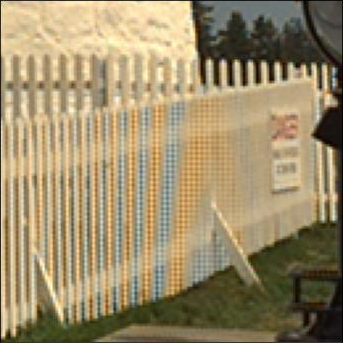
\includegraphics[width=0.5\textwidth]{figures/debayer/artifacts_gioia.png}
    \caption{Zipper effect and false colors \cite{gioiaDataDrivenConvolutionalModel2021}}
    \label{fig:artifacts_gioioa}
\end{figure}

\subsection{Malvar-He-Cutler}
\gls{mhc} pattented a simple but performant linear method using 5x5 filters that shows surprisingly good results \cite{malvarHighqualityGradientcorrectedLinear2009}.
The method they present is derived as a modification of bilinear interpolation, and it involves adding Laplacian cross-channel corrections to improve the quality of the bilinear method \cite{getreuerMalvarHeCutlerLinearImage2011}.
The demosaicking is implemented by convolution with a set of linear filters, and there are eight different filters for interpolating the different color components at different locations as can be shown in Figure \ref{fig:debayer:malvar_filters}.
Although several more sophisticated methods have been developed, the simple \gls{mhc} method works remarkably well \cite{liImageDemosaicingSystematic2008}\cite{kwanComparisonDeepLearning2019}\cite{getreuerMalvarHeCutlerLinearImage2011}.
The method is better suited for parallel execution than some others as discussed in \todo.

\subsection{Efficient separation}


\subsection{Reuse optimization}
The current \gls{mhc} method requires six lines of the image to be available in local memory for efficient operation.
Techincally it woulb be possible to use only five, but this would result in more cumb

\subsection{Separation}
The \gls{volta} has 48KiB of available shared memory per block \cite{rigerunNVIDIAJetsonXavier2023}.
With an image width of 2448 pixels \cite{lucidvisionlabsTriton0MPPolarization} it is only possible to store 10 lines in local shared memory.
\begin{align}
    \frac{48Kib}{2448px/line * 16b/px} = \frac{393216b}{39168b/l} \approx 10.039line
\end{align}
If the

\begin{figure}[H]
    \centering
    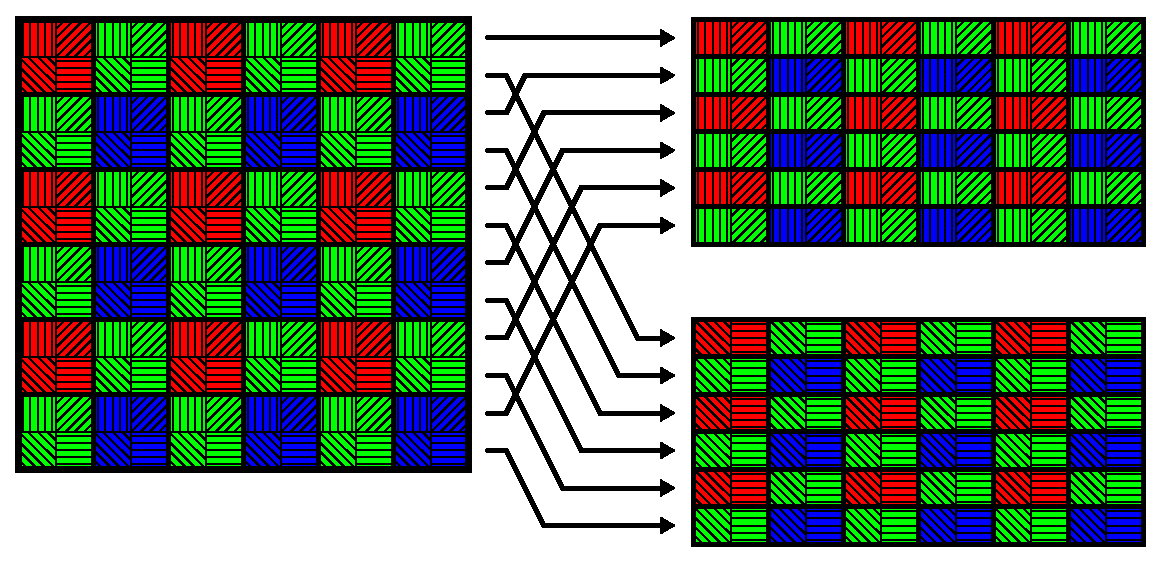
\includegraphics[width=\textwidth]{figures/debayer/separation.pdf}
\end{figure}
\subsection{Failed improvement}

\subsection{Runtime}
\begin{figure}[H]
    \centering
    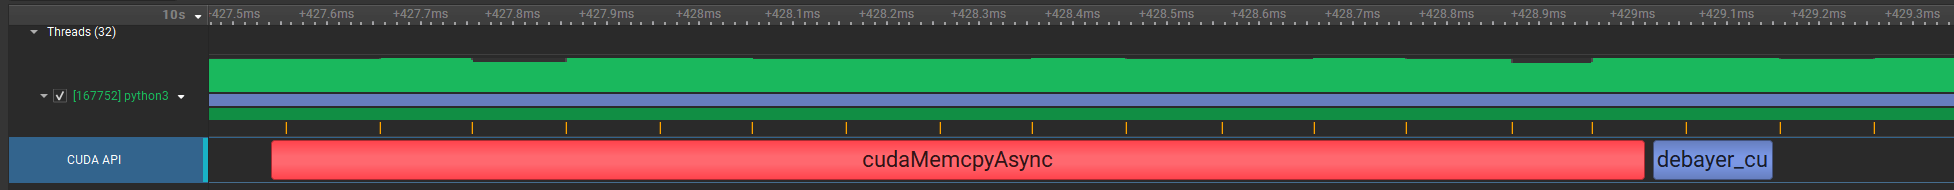
\includegraphics[width=\textwidth]{figures/memory_comparaison.png}
\end{figure}

With a runtime of $1 ms \pm 1 \mu s$
Nsight compute not working for memory

\subsubsection{Contiguous acces using warp level primitives} \label{sec:contuguous_access}
As we want to operate on 32-bit values and each pixel is stored as a 10bit value, each thread is processing 160 bits, or five words as it is the lowest common multiple of 32 and 10.
Thus every thread reads five consecutive words as shown:
\begin{align}
    a_T[i] = d[T*32+i], &  & i \in (0,1,2,3,4)
\end{align}
Where $T$ is the thread intex in the warp, $a_T$ is local memory of thread $T$, $d$ is the image stored in device memory, and $k$ is some constant offset.

It was hypothized that it would be faster to let first read the data contiguously as and then redistribute the data as follows:
\begin{align}
    c_T[i] & = d[i*32+T],        &   &                 & i & \in (0,1,2,3,4) \\
    a_T[i] & = c_j[(T*5+i)//32], & j & = (T*5 + i)\%32 & i & \in (0,1,2,3,4)
    \label{eq:contiguous_reading}
\end{align}
Where $c_T$ is local memory of thread $T$ and $//$ is the ineger division operator, i.e. $x//y = \lfloor x/y \rfloor$.
The full table of all the values in a warp are shown in Table \ref{table:memory_index} in Appendix \ref{appendix:additional_resources}.

First it was attempted copy data from device memory into shared memory as shown in eq.\ref{eq:contiguous_reading}, but this turned out to be slower.
A secont attmempt was donw using the \code{__shfl_sync} function which is a warp-level primitive used to exchange data between threads in a warp \cite{linUsingCUDAWarpLevel2018}.
As the data exchange is performed directly between registers this is faster than going through shared memory \cite{linUsingCUDAWarpLevel2018}
However instead of specifiying what data to read from what thread, as in Eq. \ref{eq:contiguous_reading}, you need specity what data to send and what thread to read from, which is more difficult.
\begin{align}
    c_T[i] & = d[i*32+T],       &   &                 & i & \in (0,1,2,3,4) \\
    c_T[j] & \rightarrow a_x[i] & j & = \todo         & i & \in (0,1,2,3,4) \\
    a_T[i] & \leftarrow c_j[x]  & j & = (T*5 + i)\%32 & i & \in (0,1,2,3,4)
    \label{eq:contiguous_reading}
\end{align}
Where $x$ represents some locally unknown variable.

\todo cache stuff test





\subsubsection{Use of constant memory}
During the development process it was tested whether storing the constant values used in the debayer algorithm in constant memory would speed up the process.
Constant memory is a type of limited read-only memory available on NVIDIA \glsps{gpu} \cite[61]{nvidiaCUDABestPractices2023}.
NVIDIA \glspl{gpu} only have 64KiB of constant memory \cite[61]{nvidiaCUDABestPractices2023}.
Read instruction from constant memory are very efficient and the best performance is acheived when all threads in a warp, as opposed to regular memory where this would result in inefficient collisions \cite[61]{nvidiaCUDABestPractices2023} \cite[13,14]{volkovLatencyHiding2016}
As the different threads in each warp would need the same constants this is ideal.

All unique constant variables used in the algorithm were collected as a part of the automatic code generation and stored in a constant device array.
Unfortynately this change had no visible impact on the performance.
A minimal test was later created that performed a very simple repeated multiply and add operation, where the coefficient and constats were either stored in constant memory or defined expicitly in the funciton as shown in \code{mfa_1} and \code{mfa_2} in Listing \ref{listing:cuda_mem_tests}.
This minimal tests showed that using constant memory was actually marginally slower (0.08\% on average) than using explicit values.

Further it was tested weither the compiled code would beform better if the values in local constant variables as in the \code{mfa_3} function in Listing \ref{listing:cuda_mem_tests}.
This gave marginally better results than \code{mfa_1} (0.04\% on average), but was deemed unecessery to implement.

\begin{listing}[H]
    \begin{minted}{cuda}
        __device__ __forceinline__ __half2 mfa_1(__half2 a) {
        return __hfma2(__float2half2_rn(0.098f), a, __float2half2_rn(3.14f));
        }
        __device__ __forceinline__ __half2 mfa_2(__half2 a) {
            return __hfma2(constant_mem[0], a, constant_mem[1]);
        }
        __device__ __forceinline__ __half2 mfa_3(__half2 a) {
            const __half2 b = __float2half2_rn(0.098f);
            const __half2 c = __float2half2_rn(3.14f);
            return __hfma2(b, a, c);
        }
    \end{minted}
    \caption{Small functions used to test local memory implementations.}
    \label{listing:cuda_mem_tests}
\end{listing}



\subsection{Better reading}
Another improvement was to use an array of pointers, rather than an array of arrays.
Initially the the section of the image on which calculations were performed were stored as an array of arrays in local shared memory.
When the computations on that part was performed, the whole block would move down.


\subsection{Half precitions floating point}
The bi



\subsection{Shortcomings}
A shortcoming of the current method is that it does not optimal gains.
Firstly the values used in \gls{mhc} are rounded to the neared dyadic rationals, to work efficently using integer arithmetic and bitshifting \cite{getreuerMalvarHeCutlerLinearImage2011}.
As the current proposed implementation uses floating point arithmetic, this rounding is disadventagious.
Another minor issues is that the values in \gls{mhc} were found to be the best fit for the well-known public-domain Kodak image set \cite{malvarHighqualityGradientcorrectedLinear2009}.
This is a set of 24 varied images, shown in Figure \ref{fig:kodak_image_suite}, that might not be the best representation of the images the \sr will capture in maritime environments.
It might be beneficial to recalculate the values based on a more representative dataset and use the floating point values rather than the rounded ones in the future.


\begin{figure}[H]
    \centering
    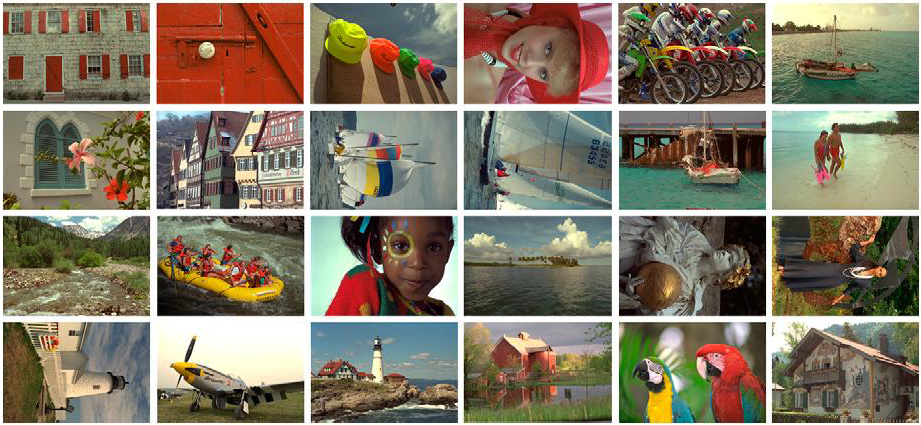
\includegraphics[width=0.8\textwidth]{figures/debayer/kodak_test_suite.png}
    \caption{Kodak image suite \cite{franzenTrueColorKodak2013}\cite{chungAdaptiveColorFilter2006}}
    \label{fig:kodak_image_suite}
\end{figure}


\begin{figure}[H]
    \centering
    \begin{tabular}[b]{ccc}
        \subcaptionbox{Exact image}{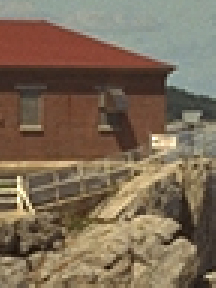
\includegraphics[width=0.3\textwidth]{figures/debayer/house_orig.jpg}}                           &
        \subcaptionbox{Observed Image}{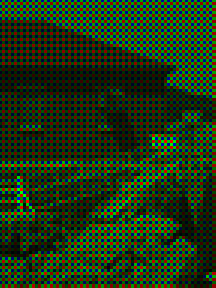
\includegraphics[width=0.3\textwidth]{figures/debayer/house_bayer.png}}                         \\
        \subcaptionbox{Bilinear (PSNR=25.61)}{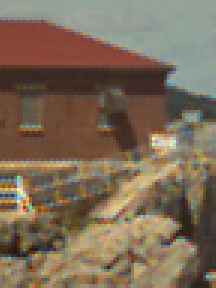
\includegraphics[width=0.3\textwidth]{figures/debayer/house_bilinear.png}}             &
        \subcaptionbox{Hamilton-Adams \todo (PSNR=31.62)}{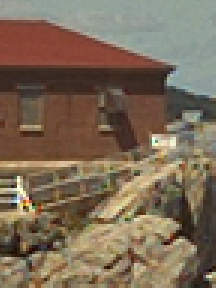
\includegraphics[width=0.3\textwidth]{figures/debayer/house_hamilton.png}} &
        \subcaptionbox{Malvar-He-Cutler (PSNR=31.15)}{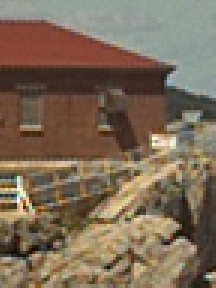
\includegraphics[width=0.3\textwidth]{figures/debayer/house_malvar.png}}
    \end{tabular}
    \caption{Coefficient values used by Malvar-He-Cutler scaled by 8 \cite{getreuerMalvarHeCutlerLinearImage2011}}
\end{figure}